% Created 2018-12-22 Sa 17:53
% Intended LaTeX compiler: pdflatex
\documentclass[11pt]{article}
\usepackage[utf8]{inputenc}
\usepackage[T1]{fontenc}
\usepackage{graphicx}
\usepackage{grffile}
\usepackage{longtable}
\usepackage{wrapfig}
\usepackage{rotating}
\usepackage[normalem]{ulem}
\usepackage{amsmath}
\usepackage{textcomp}
\usepackage{amssymb}
\usepackage{capt-of}
\usepackage{hyperref}
\author{Anton Hofmann}
\date{\today}
\title{}
\hypersetup{
 pdfauthor={Anton Hofmann},
 pdftitle={},
 pdfkeywords={},
 pdfsubject={},
 pdfcreator={Emacs 25.2.2 (Org mode 9.1.14)}, 
 pdflang={English}}
\begin{document}

\tableofcontents

\section{HOWTO git}
\label{sec:org3a6aa28}

\begin{itemize}
\item Anton Hofmann

\item \url{https://git-scm.com/book/de/v1/Git-Grundlagen-\%C3\%84nderungen-am-Repository-nachverfolgen}
\end{itemize}



\section{Intro: 4 Bereiche}
\label{sec:orged7d822}

\begin{itemize}
\item Arbeitsverzeichnis (working area)
\item Staging-Area (index oder stage)
\item local repository (committed area)
\item remote repository
\end{itemize}


\section{Intro: The big picture}
\label{sec:orgc0aa598}

\begin{itemize}
\item The Big Picture
\end{itemize}

\begin{center}
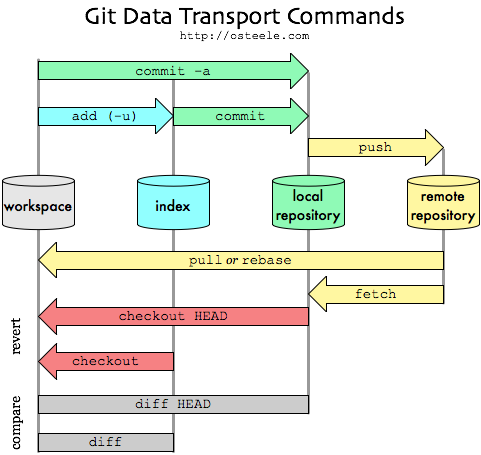
\includegraphics[width=.9\linewidth]{./img/git-tbp.png}
\end{center}


\begin{itemize}
\item Überblick und Referenz: \url{https://ndpsoftware.com/git-cheatsheet.html}
\end{itemize}

\begin{center}
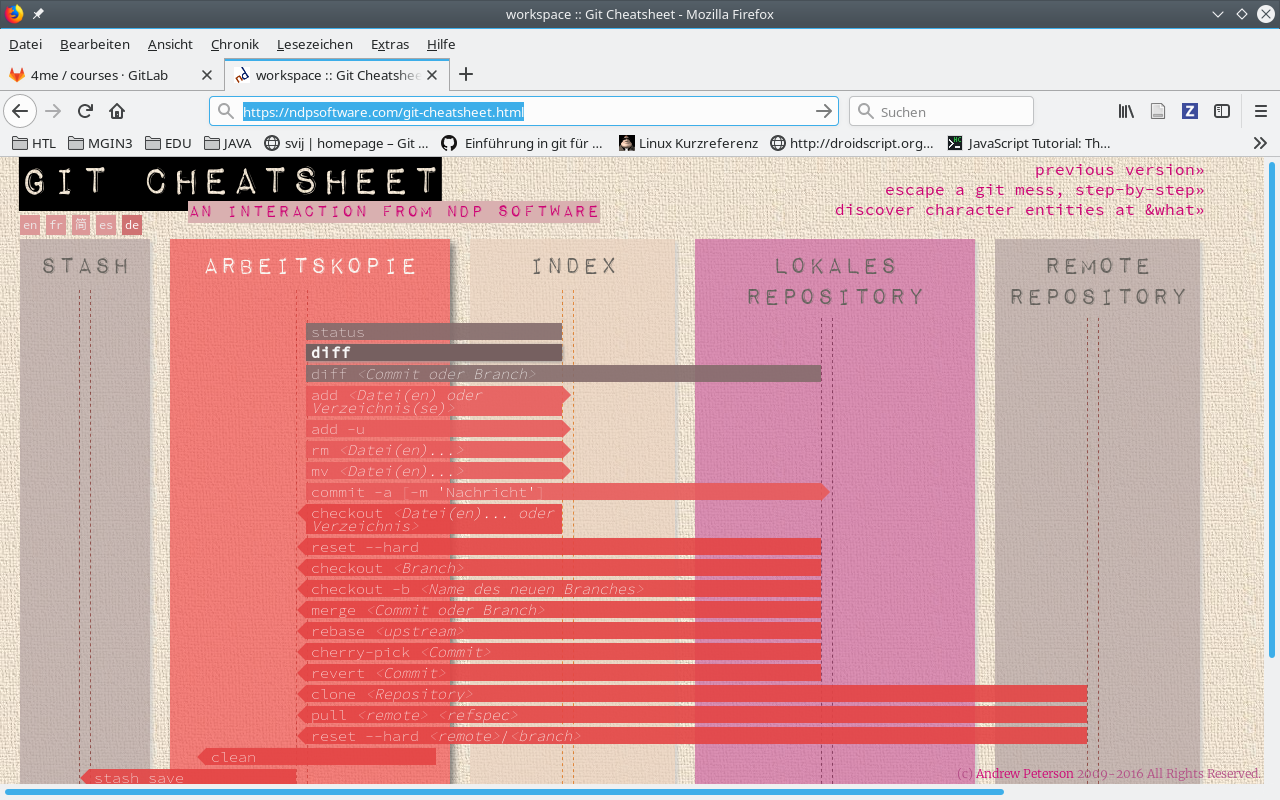
\includegraphics[width=.9\linewidth]{./img/git-overview.png}
\end{center}


\section{Übung: Config}
\label{sec:org16af1bf}

\begin{verbatim}
git config --global user.name "Anton Hofmann"
git config --global user.email "anton.hofmann@htl-salzburg.ac.at"
\end{verbatim}


\section{Übung: Eigenes Repository erzeugen und clonen}
\label{sec:org9059db0}
\begin{itemize}
\item ein repository auf gitlab.com erzeugen und clonen
\end{itemize}

\begin{verbatim}
1. auf gitlab.com ein private repository erzeugen (zB. howto-git)

2. mkdir GITlab
3. cd GITlab
4. git clone https://gitlab.com/<??your-name??>/howto-git.git
5. cd howto-git
\end{verbatim}


\section{Übung: Ein typischer Arbeitsprozess - README.md}
\label{sec:org98bc622}
\begin{itemize}
\item README.md hinzufügen
\end{itemize}

\begin{verbatim}
cd howto-git
nano README.md
git add README.md
git commit -m "add README"
git push -u origin master
\end{verbatim}


\section{Übung: Ein typischer Arbeitsprozess - .gitignore}
\label{sec:orgcf0c91e}

\begin{itemize}
\item Was soll nicht ins repository
\end{itemize}

\begin{verbatim}
cd howto-git

nano .gitignore
# Keine Executables usw.
*.exe
*.lib
*.dll 
*.log
*.class
build/
bin/
temp-*


git add .gitignore
git commit -m".gitignore"
git push -u origin master
\end{verbatim}


\section{Intro: Branching}
\label{sec:org508439c}

\begin{itemize}
\item Mehreren Commits einen Namen geben (zB: master, develop, testing, bugfix)
\end{itemize}


\begin{itemize}
\item Erzeugt einen neuen lokalen Branch \textbf{testing} und
\item wechselt in diesen
\end{itemize}
\begin{verbatim}
git branch testing
git checkout testing

oder
git checkout -b testing
\end{verbatim}


\begin{itemize}
\item Listet alle lokalen Branches im aktuellen Repository auf
\end{itemize}
\begin{verbatim}
git branch
\end{verbatim}


\begin{itemize}
\item Löscht den angegebenen Branch \textbf{testing}
\end{itemize}
\begin{verbatim}
git branch -d testing
\end{verbatim}


\section{Übung: Branching}
\label{sec:org7f7895e}

\begin{itemize}
\item Der branch \textbf{master} existiert bereits

\item erstellen Sie auch die folg. Branches:
\begin{itemize}
\item \textbf{develop, testing, bugfix}
\end{itemize}
\end{itemize}

\begin{verbatim}
cd howto-git 

git branch develop
git branch testing
git branch bugfix

\end{verbatim}


\section{Übung: add/commit file[1-3].txt}
\label{sec:org8b68f0f}

\begin{itemize}
\item Sie aktualisieren ihr lokales Repo mit \texttt{git pull}

\item Sie arbeiten auf dem branch \textbf{master}

\item Erstellen Sie nun die Dateien:
\begin{itemize}
\item \textbf{file1.txt, file2.txt, file3.txt}
\end{itemize}

\item Erzeugen Sie pro Datei je einen Commit

\item laden Sie ihre Änderungen auf gitlab mit \texttt{git push}
\end{itemize}

\begin{verbatim}
cd howto-git

git pull origin master

echo "1" > file1.txt

git add file1.txt
git commit -m"file1.txt added"

echo "22" > file2.txt

git add file2.txt
git commit -m"file2.txt added"

echo "333" > file3.txt

git add file3.txt
git commit -m"file3.txt added"

git log

git push origin master
\end{verbatim}


\begin{itemize}
\item git log liefert zum Beispiel:
\end{itemize}
\begin{verbatim}
commit 97a9298c03c1964d8aac4764bf9842746ca0803d (HEAD -> master)
Author: Anton Hofmann <anton.hofmann@htl-salzburg.ac.at>
Date:   Sun Oct 21 18:18:24 2018 +0200

	file3.txt added

commit 3d6150f68260f90d4dce55f73b54e0f5948d915b
Author: Anton Hofmann <anton.hofmann@htl-salzburg.ac.at>
Date:   Sun Oct 21 18:18:05 2018 +0200

	file2.txt added

commit 034dd5c158af7e8d4c3026c6ad080b9e1c87cb83
Author: Anton Hofmann <anton.hofmann@htl-salzburg.ac.at>
Date:   Sun Oct 21 18:17:23 2018 +0200

	file1.txt added

commit af9347d369566d8570f6856fcda5aa6b76e02c33 (origin/master, testing, bugfix)
Author: Anton Hofmann <anton.hofmann@htl-salzburg.ac.at>
Date:   Sun Oct 21 00:02:20 2018 +0200

	erstes commit

\end{verbatim}


\section{Intro: Merging}
\label{sec:org7a9a2e9}

\begin{itemize}
\item Um die Arbeiten in verschiedenen branches zusammenzufassen.

\item Einen ersten Vergleich vor dem eigentlichen \texttt{git merge} mit \texttt{git diff source\_branch target\_branch}

\item Beispiel:
\begin{itemize}
\item git checkout master
\item git diff testing master
\item git merge testing
\end{itemize}
\end{itemize}



\section{Übung: Merging ohne Konflikt - testing (add file4.txt)}
\label{sec:org172d32c}

\begin{itemize}
\item im branch testing file4.txt neu hinzufügen und
\item merge testing into master
\end{itemize}


\subsection{1. branch testing vorbereiten}
\label{sec:orga9e8ea1}
\begin{enumerate}
\item Verwenden Sie den branch \textbf{testing} und
\item fügen Sie die Datei \textbf{file4.txt} hinzu
\end{enumerate}


\begin{verbatim}
cd howto-git

git checkout testing

ls

echo "4444">file4.txt

git add file4.txt
git commit -m"file4.txt added"

git push origin testing
\end{verbatim}

\subsection{2. merge testing into master}
\label{sec:orgadd04c8}

\begin{verbatim}
git checkout master

ls

git diff testing master

git merge testing

ls

\end{verbatim}


\begin{itemize}
\item eine mögl. Ausgabe
\end{itemize}

\begin{verbatim}
hofmann@u00:/GITlab/howto-git (master>) % git merge testing  
Merge made by the 'recursive' strategy.
 file4.txt | 1 +
 1 file changed, 1 insertion(+)
 create mode 100644 file4.txt

hofmann@u00:/GITlab/howto-git (master>) % ls
file1.txt  file2.txt  file3.txt  file4.txt  README.md
hofmann@u00:/GITlab/howto-git (master>) % git status
Auf Branch master
Ihr Branch ist 2 Commits vor 'origin/master'.
  (benutzen Sie "git push", um lokale Commits zu publizieren)

nichts zu committen, Arbeitsverzeichnis unverändert

\end{verbatim}

\begin{itemize}
\item nun noch
\end{itemize}
\begin{verbatim}
git push origin master

git log
\end{verbatim}


\section{Übung: Merging ohne Konflikt - testing (update file4.txt)}
\label{sec:org018b828}

\begin{itemize}
\item im branch testing file4.txt ändern und
\item merge testing into master
\end{itemize}


\subsection{1. branch testing vorbereiten}
\label{sec:org7c35b35}
\begin{itemize}
\item edit file4.txt in branch \textbf{testing}
\end{itemize}

\begin{verbatim}
cd howto-git

git checkout testing

echo "Hallo, Welt!" >> file4.txt

git add file4.txt
git commit -m"file4.txt update"

git push origin testing
\end{verbatim}

\subsection{2. merge testing}
\label{sec:org9b29954}
\begin{itemize}
\item 
\end{itemize}
\begin{verbatim}
git checkout master

git merge testing

cat file4.txt

git push origin master
\end{verbatim}


\section{Übung: Merging mit Konflikt - master und testing (update file4.txt)}
\label{sec:org8a09aba}

\begin{itemize}
\item Branch master \textbf{und} branch testing ändern file4.txt und
\item erzeugen jeweils ein commit.
\item testing: ändere 4444 auf tttt
\item master: ändere 4444 auf mmmm
\end{itemize}

\subsection{1. branch testing und master ändern file4.txt}
\label{sec:org9c32f19}
\begin{verbatim}
git checkout testing

nano file4.txt    

git add file4.txt
git commit -m "file4.txt update again"


git checkout master

nano file4.txt

git add file4.txt
git commit -m "file4.txt update again"

\end{verbatim}


\subsection{2. merge testing - Es wird einen Konflikt geben}
\label{sec:orge78de38}

\begin{verbatim}
git checkout master
git merge testing
\end{verbatim}

\begin{itemize}
\item Hier ist der Konflikt
\end{itemize}

\begin{verbatim}
hofmann@u00:/GITlab/howto-git (master>) % git merge testing
automatischer Merge von file4.txt
KONFLIKT (Inhalt): Merge-Konflikt in file4.txt
Automatischer Merge fehlgeschlagen; beheben Sie die Konflikte und committen Sie dann das Ergebnis.
\end{verbatim}


\subsection{3. merge mit mergetool}
\label{sec:org459b99f}

\begin{enumerate}
\item config mergetool
\end{enumerate}

\begin{verbatim}
git config merge.tool vimdiff
git config merge.conflictstyle diff3
git config mergetool.prompt false
\end{verbatim}

\begin{enumerate}
\item starte mergetool
\end{enumerate}
\begin{verbatim}
git mergetool
\end{verbatim}

\begin{center}
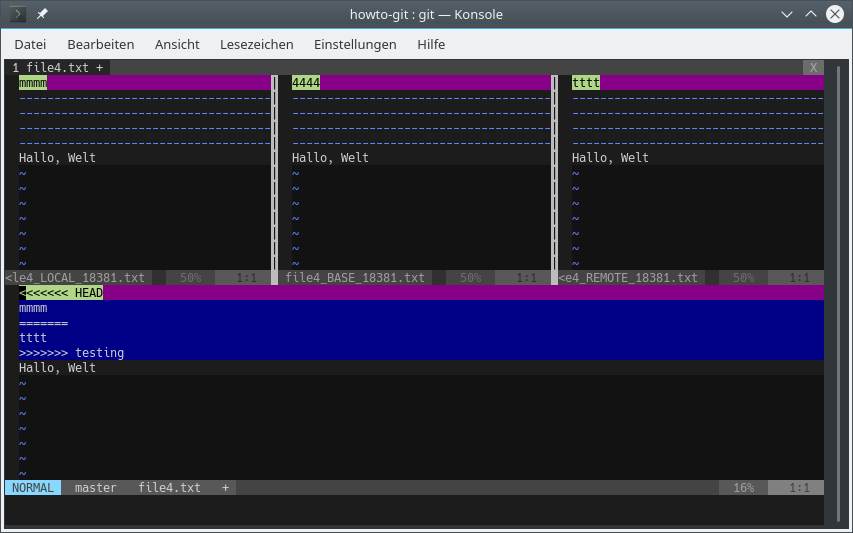
\includegraphics[width=.9\linewidth]{./img/git-mergetool-vimdiff.png}
\end{center}

\begin{itemize}
\item BASE::die Version vor dem letzten commit
\item LOCAL::die Version des aktuellen branch
\item REMOTE::die Version des zu mergenden branch
\item MERGED::die gewollte Version

\item Wählen Sie eine Version durch den Befehl
\end{itemize}
\begin{verbatim}
:diffget LOCAL
oder
:diffget BASE
oder
:diffget REMOTE

und dann editiere MERGED

und dann verlassen Sie das Tool mit
:wqa
\end{verbatim}

\begin{enumerate}
\item add und commit
\end{enumerate}
\begin{verbatim}
git add file4.txt
git commit -m"file4.txt merged with conflict"

git push origin master
\end{verbatim}


\section{Intro: Änderungen synchronisieren (lokal->remote)}
\label{sec:org8a7f96f}

\begin{itemize}
\item Austauschen der Repository-Historie

\item Pusht alle lokalen Commits zum remote (unter origin bekannt) branch (hier master)
\end{itemize}
\begin{verbatim}
$ git push origin master
\end{verbatim}


\begin{itemize}
\item Pullt die Historie vom externen Repository und integriert die Änderungen
\end{itemize}
\begin{verbatim}
git pull origin master
\end{verbatim}


\begin{itemize}
\item Lädt die gesamte Historie eines externen Repositories herunter
\end{itemize}
\begin{verbatim}
git fetch origin
\end{verbatim}




\section{Intro: Historie und Logging}
\label{sec:orgb166d71}

\begin{itemize}
\item Listet die Versionshistorie für den aktuellen Branch auf
\end{itemize}
\begin{verbatim}
git log
\end{verbatim}


\begin{itemize}
\item Listet die Versionshistorie für die aktuelle Datei auf, inklusive Umbenennungen
\end{itemize}
\begin{verbatim}
git log --follow filename.txt
\end{verbatim}


\begin{itemize}
\item Zeigt die inhaltlichen Unterschiede zwischen zwei Branches
\end{itemize}
\begin{verbatim}
git diff master testing
\end{verbatim}


\begin{itemize}
\item Gibt die Änderungen an Inhalt und Metadaten durch den angegebenen Commit aus
\end{itemize}
\begin{verbatim}
git show fb56342
\end{verbatim}


\section{Info: Arbeitsverzeichnis und die Staging-Area im Detail}
\label{sec:org6e8d91b}

\begin{itemize}
\item Listet alle zum Commit bereiten neuen oder geänderten Dateien auf
\end{itemize}

\begin{verbatim}
git status
\end{verbatim}


\begin{itemize}
\item zum \textbf{Hinzufügen} in die Staging-Area aufnehmen
\end{itemize}
\begin{verbatim}
git add filename.txt
\end{verbatim}

\begin{itemize}
\item zum \textbf{Umbennen} im Arbeitsverzeichnis und in der Staging-Area
\end{itemize}
\begin{verbatim}
git mv filename.txt filename-renamed.txt
\end{verbatim}

\begin{itemize}
\item zum \textbf{Löschen} im Arbeitsverzeichnis und in  der Staging-Area.
\end{itemize}
\begin{verbatim}
git rm -f filename.txt
\end{verbatim}


\begin{itemize}
\item zum \textbf{Verwerfen} von (falschen) Änderungen im Arbeitsverzeichnis
\end{itemize}
\begin{verbatim}
git checkout -- filename.txt
\end{verbatim}

\begin{itemize}
\item zum \textbf{Entfernen aus der Staging-Area.}
\item filename.txt \textbf{bleibt} im Arbeitsverzeichnis
\end{itemize}
\begin{verbatim}
git reset filename.txt
oder
git rm --cached filename.txt
\end{verbatim}


\begin{itemize}
\item Zeigt die Unterschiede zwischen dem Arbeitsverzeichnis und der Staging-Area
\end{itemize}
\begin{verbatim}
git diff --staged
\end{verbatim}


\begin{itemize}
\item Gibt alle derzeit indizierten Dateien permanent in die Versionshistorie auf
\end{itemize}
\begin{verbatim}
git commit -m"Ein erster Versuch der Versionierung"
\end{verbatim}


\section{Info: Commits rückgängig machen}
\label{sec:org217cc9d}

\begin{itemize}
\item Fehler beseitigen und die Historie bereinigen

\item Macht alle Commits nach dem commit fb56342 rückgängig, erhält die Änderungen aber lokal
\end{itemize}
\begin{verbatim}
git reset fb56342
\end{verbatim}


\begin{itemize}
\item Verwirft die Historie und Änderungen seit dem angegebenen Commit
\end{itemize}
\begin{verbatim}
git reset --hard fb56342
\end{verbatim}


\begin{itemize}
\item wenn die lokalen Änderungen komplett entfernen werden sollten,
\item holt man den letzten Stand vom entfernten Repository mit folgenden Befehlen:
\end{itemize}

\begin{verbatim}
git fetch origin
git reset --hard origin/master
\end{verbatim}





\section{Info: Tagging}
\label{sec:org4f3c3fd}

\begin{itemize}
\item Es wird empfohlen, für Software Releasestags zu verwenden.
\item 1b2e1d63ff steht für die ersten 10 Zeichen der Commit-Id.
\item Es können auch weniger Zeichen sein (aber eindeutig)
\end{itemize}
\begin{verbatim}
git tag 1.0.0 1b2e1d63ff
\end{verbatim}

\begin{verbatim}
git log
\end{verbatim}


\section{Info: Links}
\label{sec:orge030f4b}

\begin{itemize}
\item Visuelles: (L)
\begin{itemize}
\item \url{http://ndpsoftware.com/git-cheatsheet.html}
\end{itemize}
\end{itemize}


\begin{itemize}
\item Git (Beispiele mit bootstrap)
\begin{itemize}
\item \url{https://svij.org/blog/2014/10/25/git-fur-einsteiger-teil-1/}
\item \url{https://svij.org/blog/2014/11/01/git-fur-einsteiger-teil-2/}
\end{itemize}

\item Ein schneller Überblick:
\begin{itemize}
\item \url{http://www.nullpointer.at/2011/10/16/howto-git-commands-ein-uberblick/}
\item \url{https://rogerdudler.github.io/git-guide/index.de.html}
\end{itemize}
\end{itemize}


\begin{itemize}
\item Git-Book:
\begin{itemize}
\item \url{https://git-scm.com/book/de/v1/Git-Grundlagen}
\item \url{http://gitbu.ch/pr01.html}
\end{itemize}
\end{itemize}





\section{Info: Weitere Themen}
\label{sec:orgc9dc4ce}
\subsection{Aufschieben und Wiederherstellen unvollständiger Änderungen}
\label{sec:org6589e1b}

\begin{itemize}
\item Speichert temporär alle getrackten Dateien mit Änderungen
\end{itemize}

\begin{verbatim}
git stash
\end{verbatim}

\begin{itemize}
\item Stellt die zuletzt zwischengespeicherten Dateien wieder her
\end{itemize}
\begin{verbatim}
git stash pop
\end{verbatim}

\begin{itemize}
\item Listet alle zwischengespeicherten Änderungen auf
\end{itemize}
\begin{verbatim}
git stash list
\end{verbatim}

\begin{itemize}
\item Verwirft die zuletzt zwischengespeicherten Änderungen
\end{itemize}
\begin{verbatim}
git stash drop
\end{verbatim}

\subsection{Beispiel: Branching and Merging}
\label{sec:orga77eb02}

\begin{itemize}
\item \url{https://git-scm.com/book/en/v2/Git-Branching-Basic-Branching-and-Merging}

\item Let’s go through a simple example of branching and merging.
\item You’ll follow these steps:
\begin{itemize}
\item Do some work on a website.
\item Create a branch for a new story you’re working on.
\item Do some work in that branch.
\end{itemize}

\item At this stage, you’ll receive a call that another issue is critical and you need a hotfix.
\item You’ll do the following:
\begin{itemize}
\item Switch to your production branch.
\item Create a branch to add the hotfix.
\item After it’s tested, merge the hotfix branch, and push to production.
\item Switch back to your original story and continue working.
\end{itemize}
\end{itemize}
\end{document}
